%%%%%%%%%%%%%%%%%%%%%%%%%%%%%%%%%%%%%%%%%%%%%%%%%%%%%%%%%%%%%%%%%%%%%%%%%%%%%%%%
% Design
%%%%%%%%%%%%%%%%%%%%%%%%%%%%%%%%%%%%%%%%%%%%%%%%%%%%%%%%%%%%%%%%%%%%%%%%%%%%%%%%
% In this section, illustrate the hardware and software interface for the
% design. Note that the most important part of the hardware design is
% parallelism, so it is important to mention how this was achieved.
\subsection{Design}
\begin{frame}{Performance Considerations}
    \note<1>{In the design of the hardware implementation, there are several
        considerations that were made in an effort to maximise the performance
        of the design.}
    \begin{itemize}
        \item<2-> Cannot transfer data faster than $O(n)$.
        \note<2>{We cannot transfer data faster than $O(n)$. This means that
            even if I were able to improve the algorithm to have a run time
            complexity of less than order $n$, the performance (and, indeed, the
            scalability) of the implementation would not significantly improve.

            Ideally, the design must minimise the number of data transfers that
            are required.}

        \bigskip
        \item<3-> For each vector that is pruned from the block, we save (on
            average) $\frac{block\_size}{2}$ distance computations.
        \note<3>{Pruning a vector from the block reduces the number of calls to
            the \escape{distance_squared} function that are required. The exact
            number of \escape{distance_squared} calculations that are prevented
            by pruning a vector the block depends on the location of that vector
            within the block.

            On average, pruning a vector from the current block will reduce the
            total number of calls to the \escape{distance_squared} function by
            $\frac{block\_size}{2}$. This is evidence that the block size has a
            significant effect on algorithm performance and must be carefully
            selected for a class of data sets.}
    \end{itemize}
\end{frame}

\begin{frame}[label=design]{Features}
    \begin{itemize}
        \item<1-> Majority of the \escape{TopN_Outlier_Pruning_Block} function
            performed in software.
        \note<1>{Based on my benchmarks of the selected algorithm, it was decided
            that the majority of the algorithm could be efficiently computed in
            software.}

        \item<2-> Computation of expensive \escape{distance_squared} function
            performed in hardware. Speed-up would be achieved by:
        \note<2>{The \escape{distance_squared} function, however, was selected
            as the top level function for a hardware implementation. This
            function single-handedly accounts for the majority of the total
            execution time of the anomaly detection algorithm, and also gives
            way to a simplistic and logical hardware implementation.

            Algorithm speed-up would be achieved by:}
        \begin{itemize}
            \item<3-> Multiple functional units.
            \note<3>{Multiple functional units. The \escape{distance_squared}
                function was designed as a functional hardware unit. The use of
                multiple \escape{distance_squared} functional units allowed for
                instruction level parallelism within the design, at the cost of
                software overhead required to manage this concurrency.}

            \item<4-> Pipelined design.
            \note<4>{Pipelined design.}

            \item<5-> Separate functional units for loading ``outer'' and
                ``inner'' vectors through DMA bus.
            \note<5>{Separate functional units for transferring the ``inner''
                and ``outer'' vectors through the DMA bus, avoiding the repeated
                DMA transfer of the same vector element.}
        \end{itemize}

        \item<6-> Software algorithm modified so as to utilise hardware
            implementation.
        \begin{itemize}
            \item<6-> Software can begin to process the next block element whilst
                waiting for \escape{distance_squared} computation to complete.
            \item<6-> Thread management and interrupt facilities required (with
                additional overhead).
            \item<6-> Increased instruction-level parallelism.
        \end{itemize}
        \note<6>{In order to accommodate the parallelism through multiple
            functional units, the software need be support by thread management
            and interrupt facilities.}
    \end{itemize}
\end{frame}

\begin{frame}<1-2>[label=design-diagram]{Diagram}
    \maxsizebox{\textwidth}{0.85\textheight}{
        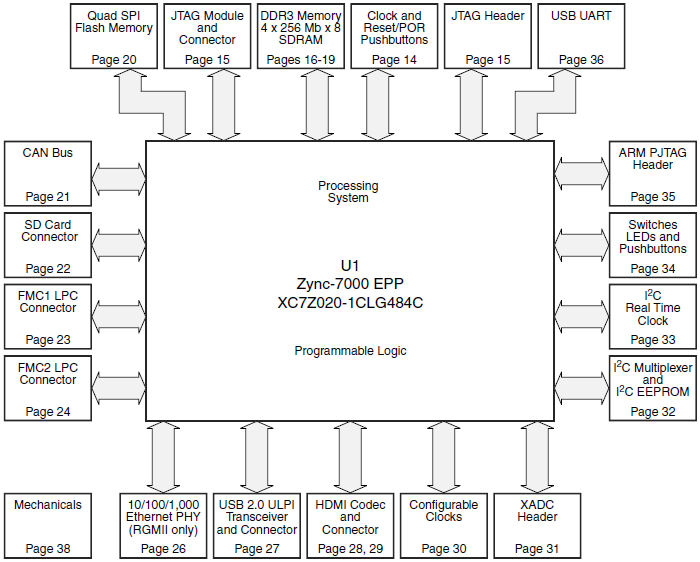
\includegraphics{design/block-diagram}
    }
    \note<1>{This diagram shows illustrates the architecture of my proposed
        design.

        The design consists of a simple ``outer vector'' group (shown on the
        left), which comprises a single hardware PCORE and a DMA module through
        which it receives data. This functional group is used to load a store a
        single vector which appears in an outer `for' loop in the implemented
        algorithm. The vector stored in this unit is compared to many other
        vectors in order to calculate the distance squared. These vectors are
        handled by the functional groups appearing on the right hand side of the
        diagram.}
    \note<2>{The ``inner vector'' groups receive a vector from the ARM processor
        through a DMA transfer. They also stream the elements of the outer
        vector through a common bus interface, shown in the middle.

        The hardware interacts with the ARM processor through an AXI
        interconnect block, shown in blue.

        The use of multiple ``inner vector'' functional unit provides great
        potential for an improvement to the algorithm execution speed. Setting
        the number of ``inner vector'' functional units to the block size
        (40 in our examples), it is possible to process the complete block of
        vectors simulatenously, excluding the software overhead required to
        manage these concurrent processes.}
\end{frame}

%%%%%%%%%%%%%%%%%%%%%%%%%%%%%%%%%%%%%%%%%%%%%%%%%%%%%%%%%%%%%%%%%%%%%%%%%%%%%%%%
% Results
%%%%%%%%%%%%%%%%%%%%%%%%%%%%%%%%%%%%%%%%%%%%%%%%%%%%%%%%%%%%%%%%%%%%%%%%%%%%%%%%
\subsection{Results}
\begin{frame}{Performance Estimates}
    The execution time for the proposed design is estimated to be the sum of:
    \begin{enumerate}[<+->]
        \item Execution time of software implementation, excluding the
            distance\_squared function
        \item Time required for DMA transfer of ``outer'' vector.
        \item Time required for DMA transfer of ``inner'' vector.
        \item The time required for the hardware to complete the computation and
            return the result.
        \item Overheads associated with thread management.
    \end{enumerate}
\end{frame}

%%%%%%%%%%%%%%%%%%%%%%%%%%%%%%%%%%%%%%%%%%%%%%%%%%%%%%%%%%%%%%%%%%%%%%%%%%%%%%%%
% Discussion
%%%%%%%%%%%%%%%%%%%%%%%%%%%%%%%%%%%%%%%%%%%%%%%%%%%%%%%%%%%%%%%%%%%%%%%%%%%%%%%%
\subsection{Discussion}
\begin{frame}[label=discussion]{Discussion}
    \begin{itemize}
        \item<1-> Execution time comparison:
        \begin{itemize}
            \item<1-> \textbf{Hardware:} $8.71 ns/cycle \times 264 cycles = 2.30 \mu s$
            \item<1-> \textbf{Software:} $1.63 \mu s$
        \end{itemize}
        \note<1>{Initial testing on the hardware design revealed that the
            hardware could only perform distance calculations at around half of
            the speed that the software calculation was capable of (and this
            neglects any additional overheads such as DMA transfer times).

            However, these figures do not portray the fact that the hardware
            implementation can be parallelised, and that tens to hundreds of
            \escape{distance_squared} functional units would comprise the
            design.

            Additionally, no attempt was made to decrease the latency of the
            hardware design or the clock period, although doing so would see a
            reduction in the execution time of the hardware implementation.}

        \bigskip
        \item<2-> Maximum expected improvement is dictated by Amdahl's Law.
        \note<2>{Amdahl's Law loosely states that speed-up of a program using
            multiple processors in parallel computing is limited by the time
            needed for the sequential fraction of the program.

            In this application, Amdahl's Law proves to be problematic for data
            transfer, which cannot be parallelised without an increase in
            resources. Therefore, it is highly likely that future effort will be
            required to further minimise the number of data transfers required
            under this design.}
    \end{itemize}
\end{frame}